% Created 2016-12-13 Tue 11:10
% Intended LaTeX compiler: pdflatex
\documentclass[11pt]{article}
\usepackage[utf8]{inputenc}
\usepackage[T1]{fontenc}
\usepackage{graphicx}
\usepackage{grffile}
\usepackage{longtable}
\usepackage{wrapfig}
\usepackage{rotating}
\usepackage[normalem]{ulem}
\usepackage{amsmath}
\usepackage{textcomp}
\usepackage{amssymb}
\usepackage{capt-of}
\usepackage{hyperref}
\usepackage{fullpage}
\usepackage{algorithm}
\usepackage{algpseudocode}
\author{sorrow17}
\date{\today}
\title{}
\hypersetup{
 pdfauthor={sorrow17},
 pdftitle={},
 pdfkeywords={},
 pdfsubject={},
 pdfcreator={Emacs 25.1.1 (Org mode 9.0.1)}, 
 pdflang={English}}
\begin{document}

\title{EECS 587 Term Project: GPU-accelerated Rigid Body Dynamics System Simulation}
\author{Zhengxu Chen \quad zhxchen@umich.edu}

\maketitle

\section{Motivation}
\label{sec:org55df02d}
I am currently making a 3d computer game engine in my undergraduate senior year. As a game player, I know there are more and more games adopting physics engines that can perform very real effects for the interacting objects in game scenes. Physics engines typically have a high cost because they usually involve intensive linear algebra calculation, and collision detection process for rigid bodies is a pain point as well. For now, there is no well-described way in open source physics engine to utilize the power of GPUs fully, so I think it might be a good idea to explore a way to accelerate physics simulation computing myself.

\section{Problem Statement}
\label{sec:org95fcb18}
Firstly, the concept of "Rigid Body" in this report needs to be defined. A "Rigid Body" is an object that has two attributes: \emph{dynamics} and \emph{shape} (or model). A dynamics attribute describes the position, momentum, rotation, angular momentum and so on of a given object. The shape describes the physics occupation of the specific object. Both attributes are defined in 3-dimensional space in this project. Baraff(1997) described a very handy way to represent the dynamics attribute of an object as follows:

\begin{verbatim}
struct Dynamics {
float mass;
float X[3]; // position of the obeject.
float R[3][3]; // rotation matrix
float P[3], // momentum
      L[3]; // angular momentum
float I_inv[3][3]; // inverse of the inertia tensor.
float F[3], // force
      T[3], // torque
};
\end{verbatim}
\captionof{figure}{Essential data members for a dynamics attribute.}

For the shape attribute, the most intuitive way is to firstly divide the surface of an object into small triangles, and store all the vertex coordinates in a list, then construct another table for indexing the vertices for each face of a triangularized object.

\begin{figure}[htbp]
\centering
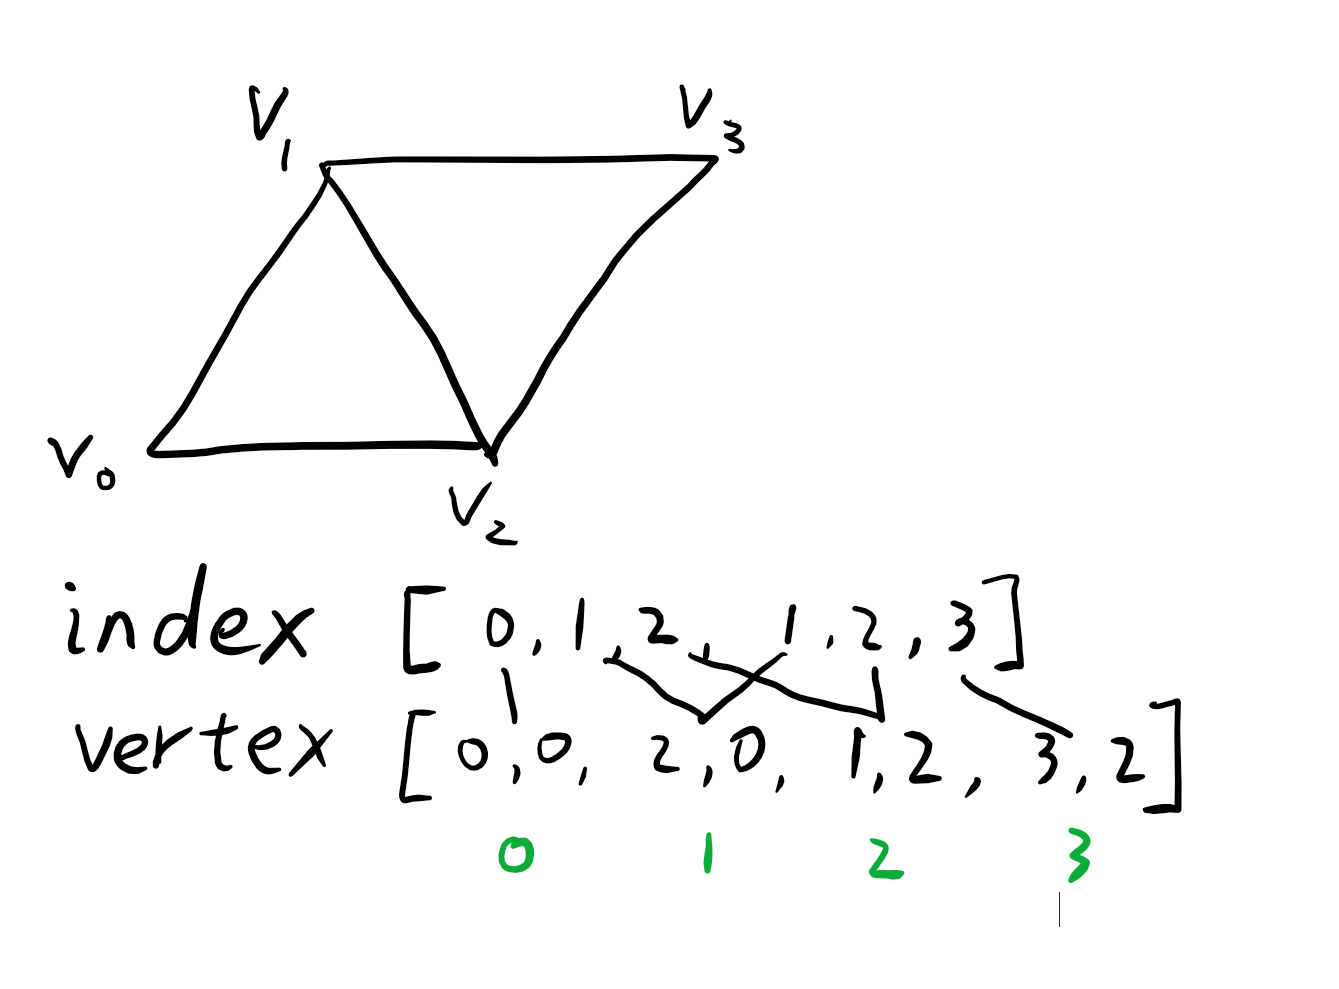
\includegraphics[width=10cm]{./rep_2.png}
\caption{A conventional way to represent shape attribute.}
\end{figure}

\subsection{Simulation Procedure}
\label{sec:orge64320e}
During the simulation procedure, given the set of objects, we simply do one thing: updating the dynamics attributes. Since shapes are immutable for rigid bodies, we do not need to update them. In this problem, we will set a fixed time interval (1/30 second) to represent the time past in the scene we are simulating after each update. In this project, we would focus on the average calculation time for each update.

\begin{figure}[htbp]
\centering
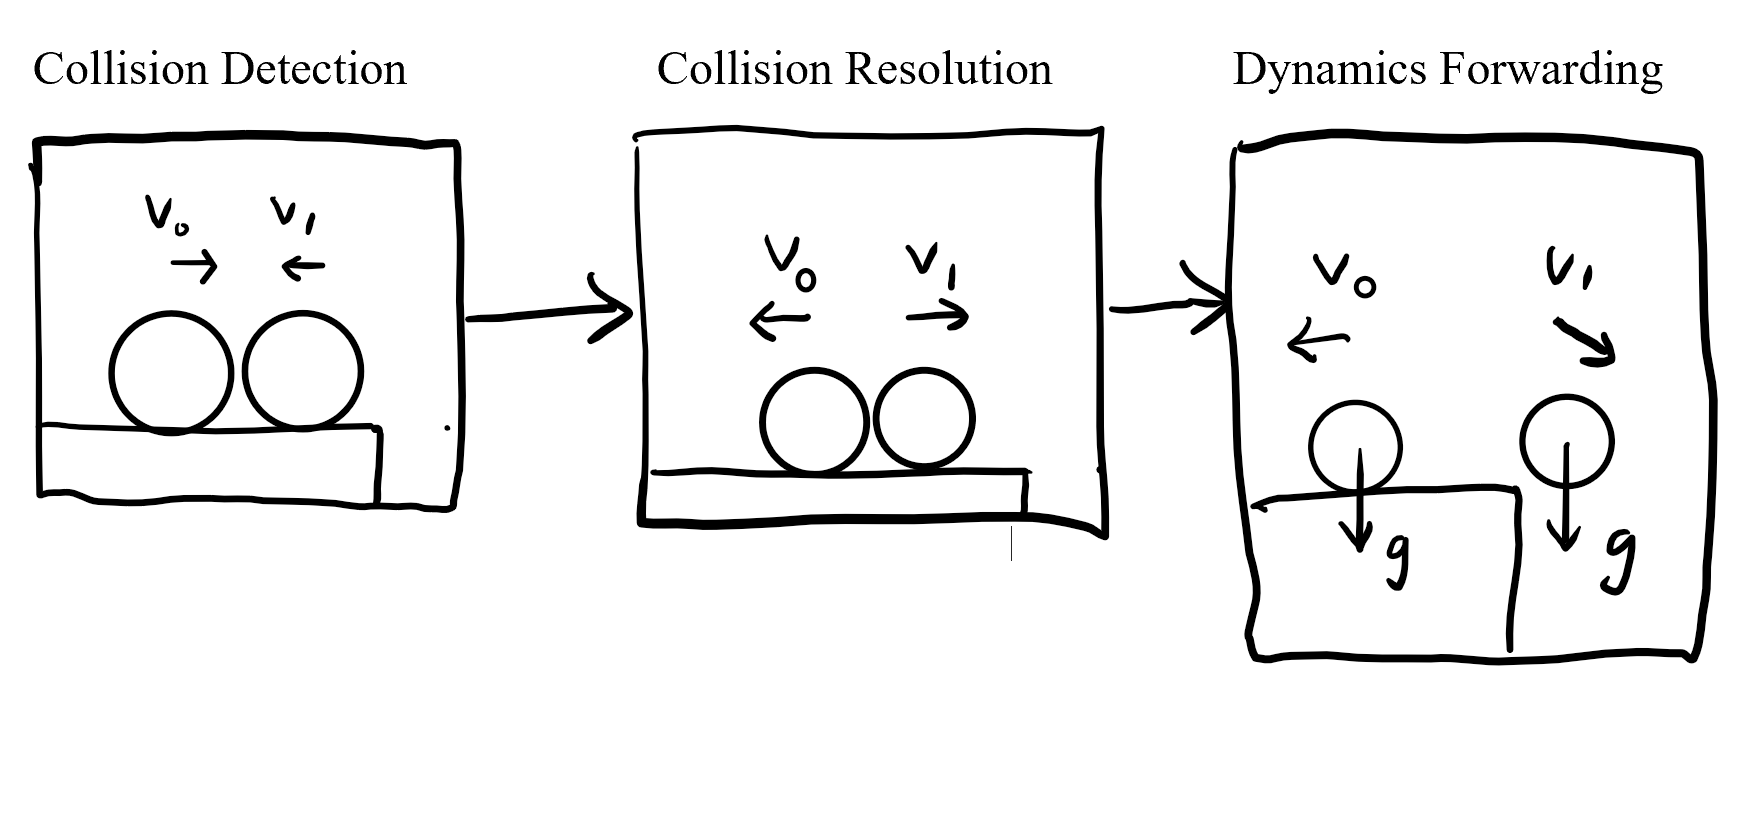
\includegraphics[width=.9\linewidth]{./rep_3.png}
\caption{General physics simulation pipeline.}
\end{figure}

Generally, at the beginning of each update, we need to detect all the object pairs that are colliding in the space based on both dynamics and shape attribute, then we should resolve these collisions by re-assigning the dynamics attribute of each object. Finally, we need to apply Newton's Law to each object to figure out the position and velocity in the next "frame," which is often called \emph{Dynamics Forwarding}. The details of each simulation phase will be discussed later.

\subsection{Benchmark}
\label{sec:org32c8596}
To measure the performance, I construct a close physics environment, which I would like to call "Box Collider." In this benchmark, a 100x100x100 sized box is set up, and there are spheres with different radius dropped into it. The balls will also bounce back when they collide with one inner face of the box.

The metrics here is to see how long would the program take for each update. I use only spheres here to simplify the problem I am going to solve so that I can focus more on the performance aspect of this project.

\begin{figure}[htbp]
\centering
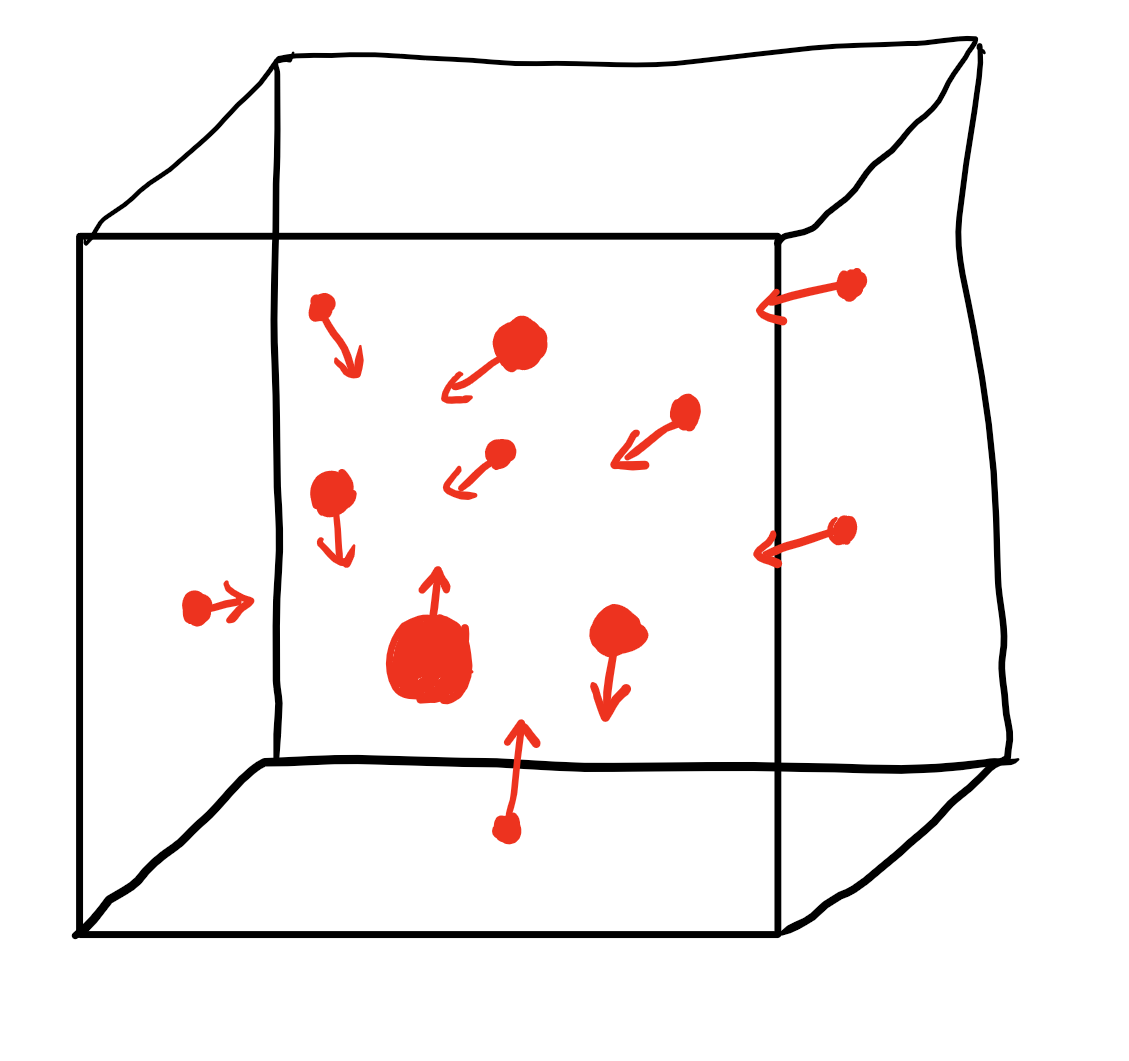
\includegraphics[width=6cm]{./rep_4.png}
\caption{The "Box Collider" benchmark (the results are not visualized yet in this project due to the complexity of setting up renderer).}
\end{figure}

I use triples --- (N, B, T) to present the input size, which indicates we are dropping N spheres in the box and using B blocks and T threads (per block) in GPU. The radiuses of spheres are uniformly distributing from 0 to 5 (of unit length).

\section{Solutions}
\label{sec:org882432b}
I will firstly describe my problem-solving procedure, the performance bottleneck I met, and how I overcame them. Then the benchmark result is shown in the next section.
\subsection{The Easy Part --- Dynamics Forwarding}
\label{sec:orgc858847}
Given the dynamics attribute of an object, and the force and torque enforced, we can just apply Newton's Law, and I will briefly describe the update procedure as the following: 

\begin{algorithm}[H]
\begin{algorithmic}[1]
\Procedure{ForwardDynamics}{Object, dt}
\State $O \gets Object$
\State $O.Momentum \gets O.Momentum + dt\cdot O.Force$
\State $O.AngularMomentum \gets O.AngularMomentum + dt\cdot O.Torque$
\State $O.Velocity \gets O.Momentum/O.Mass$
\State $O.Position \gets O.Position + dt\cdot O.Velocity$
\State $O.Rotation \gets UpdateRotation(O.Rotation, O.AngularMomentum)$
\EndProcedure
\end{algorithmic}
\end{algorithm}

As we can see this operation can be easily parallelized on objects respectively, since the state of each object is independent at this stage. Note that we are assuming the collision has been resolved in this phase.

\subsection{The Hard Part --- Collision Handling}
\label{sec:orgd5a72f1}

\subsubsection{A Naive Approach}
\label{sec:orgfe8286c}
In physics simulation, we want to detect all the intersecting object pairs and then update the dynamics attribute after the collision for them. A naive algorithm to do this is like:

\begin{algorithm}
\begin{algorithmic}[1]
\Procedure{DetectCollision}{ObjectSet}
\State $answers \gets \{\}$
\For {$ a, b \gets \text{AllPairs}(ObjectSet) $}
\If {$ HaveIntersection(a, b)$}
\State $answers \gets answers \cup \{(a, b)\}$
\EndIf
\EndFor
\State
\EndProcedure
\end{algorithmic}
\end{algorithm}

Obviously, the time complexity of this algorithm is O(n\(^{\text{2}\cdot}\) T(HaveIntersection)). In general, this algorithm can be easily parallelized because each object pair is independent of others. We just need to encode each object pair and assign the pairs to GPU threads in parallel. To give an intuitive impression on how slow this parallel algorithm is, I will provide the performance measurement briefly here:

\begin{table}[htbp]
\centering
\begin{tabular}{rrrrrrr}
Objects(N) \# & Blocks(B) \# & Threads(T)/Block \# & Time(ms) & B \# & T/Block \# & Time(ms)\\
\hline
100 & 16 & 16 & 0.2933 & 8 & 64 & 0.1859\\
500 & 16 & 16 & 5.3388 & 8 & 64 & 2.8176\\
1000 & 16 & 16 & 21.8844 & 8 & 64 & 11.0379\\
5000 & 16 & 16 & 534.405 & 8 & 64 & 273.7910\\
\end{tabular}
\caption{Performance of brute force pairing enumerating method. (measured with Nvidia\textregistered GTX 940M graphics card, which has 384 processing units and 1072MHz clock cycle.)}

\end{table}

Since typically a game engine needs to refresh the dynamics attribute of an object in the frequency of 30Hz (or 60 Hz), when the number of objects goes up, the time that required to detect collisions is skyrocketing. Players can only afford the cost of calculation when object number is less than 100 with their PC level graphics card (in my case, it is Nvidia GTX 940M with 384 shaders). Therefore we must find other ways to solve this problem.

\subsubsection{Broad Phase Collision Pair Elimination}
\label{sec:orge4138f9}
A more common way to do collision detection is a two-phase procedure, which named \emph{broad phase} and \emph{narrow phase} respectively. In a collision detection broad phase, we want to eliminate most of the object pairs that apparently cannot collide. For example, two spheres with unit length radius that are 100 unit length away from each other should not even be considered in our scenario. But how can we eliminate very distant object pairs in advance?

\begin{figure}[htbp]
\centering
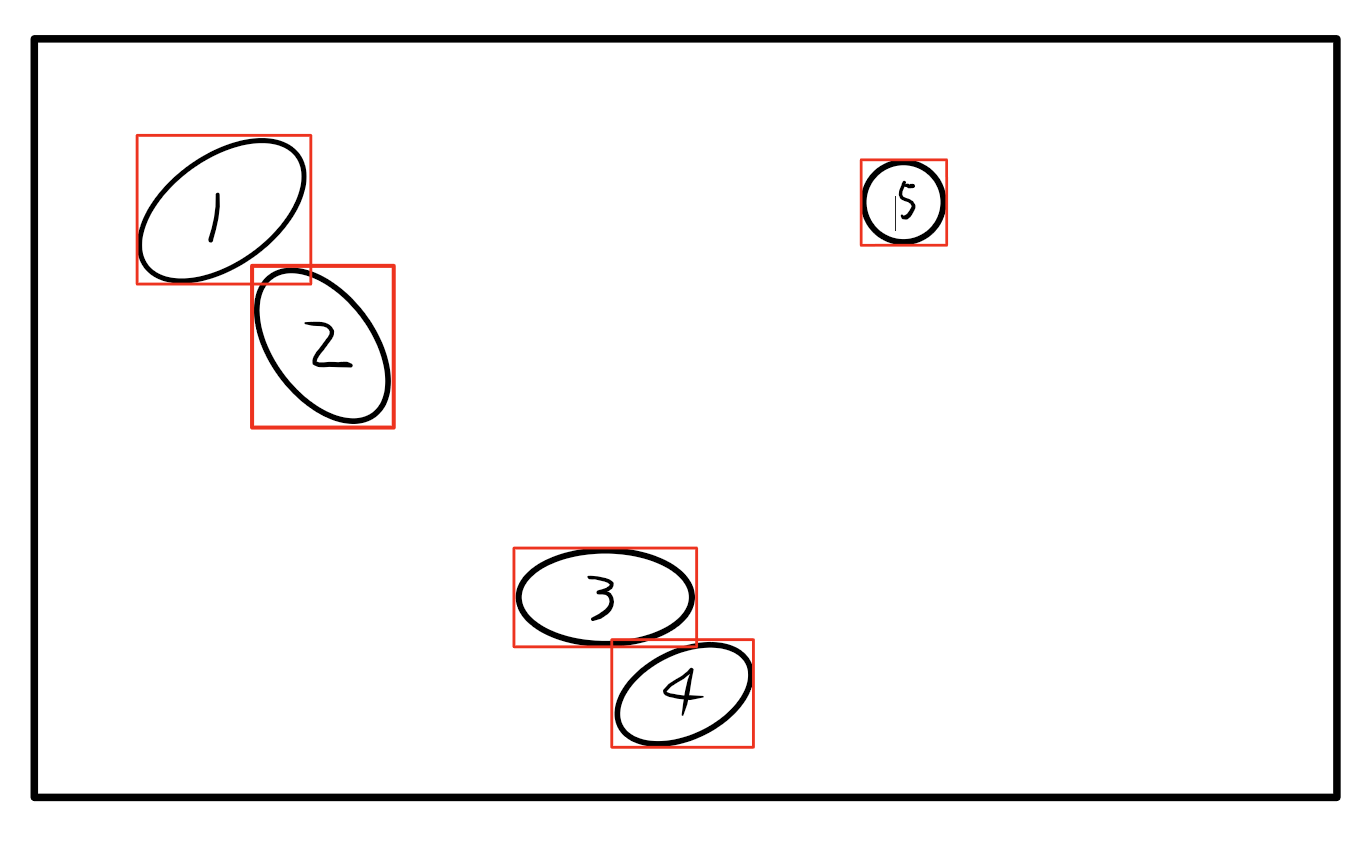
\includegraphics[width=8cm]{./rep_5.png}
\caption{Broad phase collision detection. We should filter out all the object pairs that apparently can not collide, and only leave the pairs "might collide," like (1,2) and (3,4) in the scene. Totally there are ten unordered pairs in the scene, so this would be very useful in practice.}
\end{figure}

The answer would be to maintain a data structure that entails this type of information. When we are considering using spatial information based data structures, it is important to note that:
\begin{itemize}
\item It must be easy to build in code because we can only implement limited types of logic on GPU compared to CPU.
\item It must be suitable for parallelization since we want to utilize the power of GPU entirely.
\item It should be cheap to maintain and construct in GPU, and fast in general.
\end{itemize}
Otherwise we would waste a lot of time on inappropriate data structures implementation, finally finding the performance is awful.

In our case, there are four choices that worth trying:
\begin{itemize}
\item Uniform grid
\item K-d tree
\item Binary Space Partitioning
\item Boundary Volume Hierarchy
\end{itemize}

Let's compare them in the following table:
\begin{center}
\begin{tabular}{llll}
Data Structure & Easy to Implement? & Parallelizable? & Cheap and Fast?\\
\hline
Grid & Yes & Yes & Mostly not\\
K-d tree & No & Yes & Not for moving objects\\
Binary Space Partitioning & No & Yes & Yes (in time complexity)\\
Boundary Volume Hierarchy & Yes & Yes & Yes (in practice)\\
\end{tabular}

\end{center}

Considering these aspects, I decided to use Boundary Volume Hierarchy (BVH) as the data structure.

\subsubsection{Data Structure Construction}
\label{sec:orgf732fa3}
Then it is necessary to think about another question: Should we construct the data structure in the first frame and maintain it in the following frames, or is it better to build the data structure from scratch in each frame? It seems that the first approach would cost less but indeed it does not. The reason is that maintaining a balanced BVH tree here might be fast on CPU, but it cannot be easily parallelized on GPU, especially when there are hundreds of shaders present. In \emph{Bullet3d} physics engine, a random deletion and insertion procedure is adopted to keep the BVH balanced, but it does not quite fit in this problem since all of the maintaining algorithms will cause a lot of cache misses inside GPU blocks when trees are organized in linked structure. It is more convenient and fast just to rebuild BVH each frame using GPU. I used Axis-aligned Minimum Bounding Box (AABB) as the Boundary Volume Hierarchy here as it usually is good enough for performance.

In EECS 587: Parallel Computing lectures, we have discussed topics about space filling curves, which can be naturally applied to this situation. In BVH, the order of leaf nodes that we traverse is not specified by BVH itself. We can construct a BVH in arbitrary order of leaf nodes. However, as we can see in the following figure 6, if we cannot "cluster" nearby objects together, then there will be quite a lot of spaces overlap among the bounding boxes. Hence we need a method to map all the objects into an ordered list, such that when two objects are close enough in the space, they are also close enough in the list.

\begin{figure}[htbp]
\centering
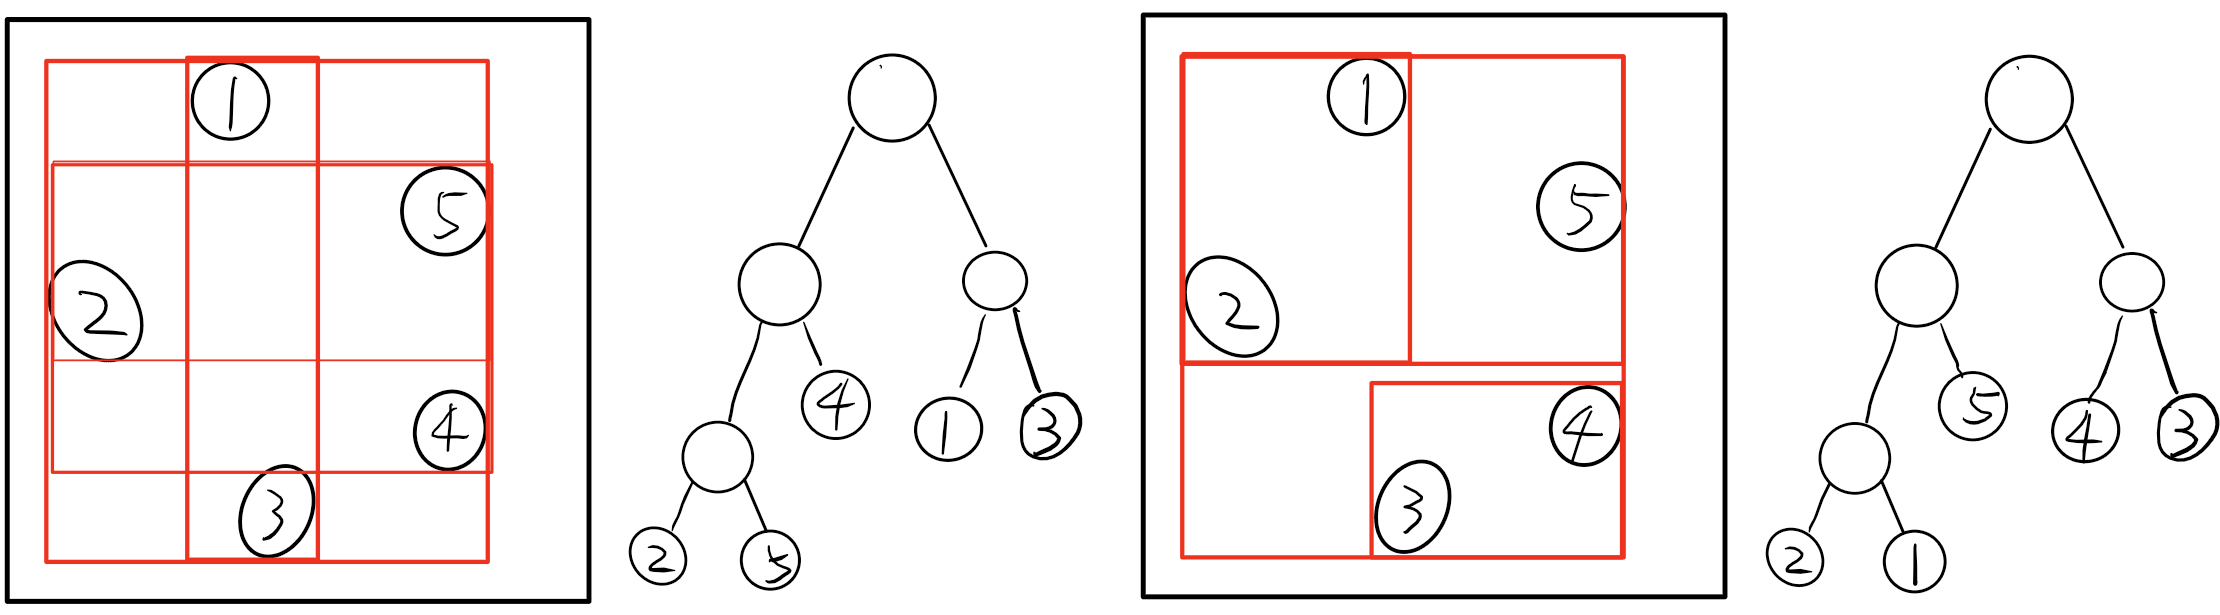
\includegraphics[width=.9\linewidth]{./rep_6.png}
\caption{Unclustered BVH (left) vs. clustered BVH (right). A query needs to traverse much more nodes than the clustered version.}
\end{figure}

Evidently, we can use a z-ordering space filling curve to accomplish that. To construct the ordered list, I used a well-developed algorithm called Radix Sort, which is the state-of-art parallel sorting algorithm on GPU. Harada and Howes (2011) gave a nice introduction to it.

In fact, the approach to use an ordered list is what Lauterbach and Luebke (2007) proposed in the paper "Fast BVH Construction on GPUs." This method can generate a well-formed tree with relatively low cost. I do use this idea to organize the order of each object, but finally, I decided not to use their way to construct the actual tree, as it still has a lot to improve in performance aspect when it comes to "Box Collider" environment which I used for benchmarking. In their paper, a top-down way is used to build the tree from a root node. The basic idea is to maintain a working queue storing intervals in the z-ordering list and let GPU shaders to divide up those intervals in parallel, like what the students did in EECS 587 homework 4 (if they used a BFS approach). This method can be applied to many super-intensive object settings, like cloth simulation context. In fact, when it comes to "box collider" model, it still has overhead which can hurt the parallelization sometimes. The reason might be that there are too much data communication between blocks to synchronize the working queue here. (I will briefly show it in the "Performance" section.)

Then I recalled the golden principle "Keep it Simple and Stupid." The objective I want to achieve is simple here. I just need a fast-constructed balanced AABB tree per frame. Therefore I began to think the "bottom-up" way to construct the tree. The bottom-up way is like the following figure:

\begin{figure}[htbp]
\centering
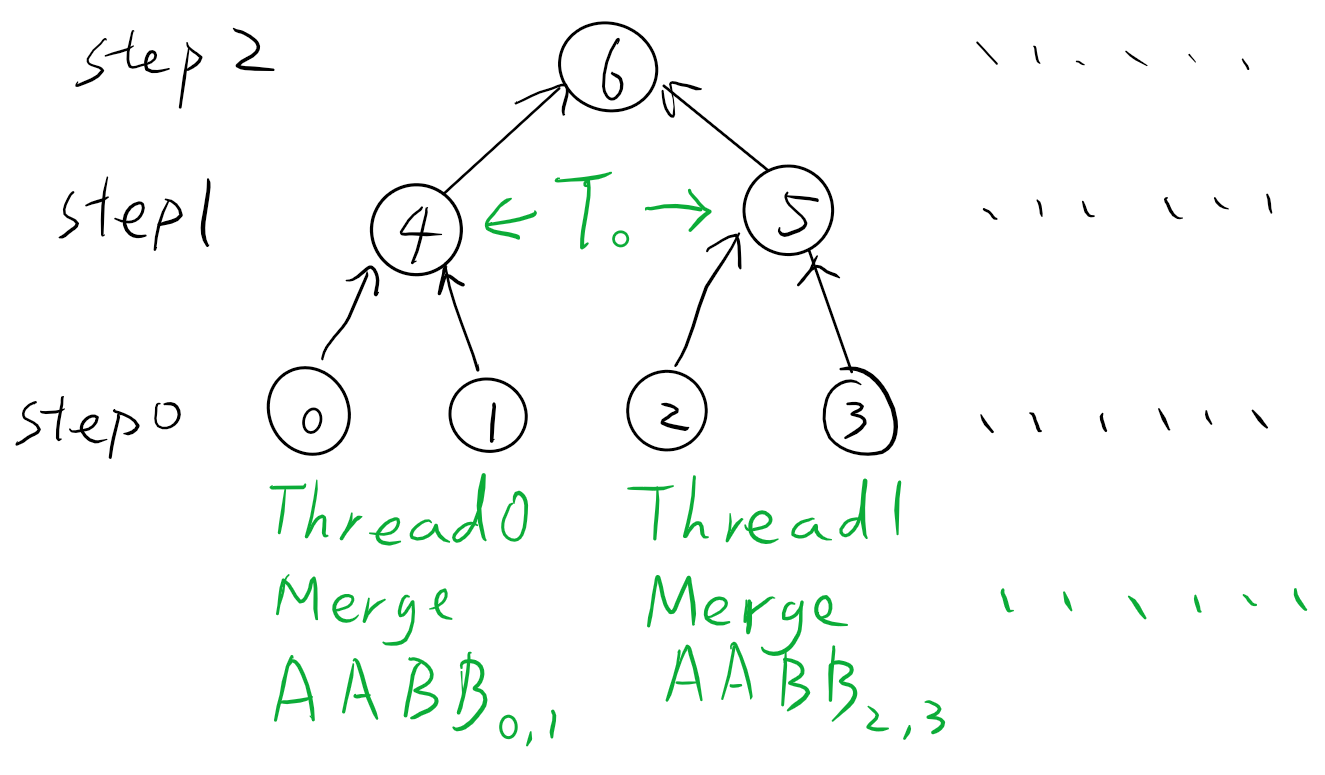
\includegraphics[width=10cm]{./rep_7.png}
\caption{Bottom-up way to construct a BVH tree. In the figure, thread zero will merge the AABBs of node 0 and 1; the thread one will merge AABBs for the next two nodes,  and so on. When the current level is fully merged, we synchronize all the threads for only once and let them repeatedly merge every two consecutive nodes in the next step.}
\end{figure}

The advantage of this approach is that we are constructing the tree level by level from the deepest leaf nodes, and on each level of the construction, processors have already known the nodes they are going to handle, without any synchronization method, such as a working queue. Again, there are good reasons for Lauterbach and Luebke to do that, but in this case, this bottom-up way is faster and scales well.

The time complexity of bottom-up construction should be O(log n) in the worst case, as a balanced BVH tree has at most log(n) levels.

\subsubsection{Top Down BVH Traversal}
\label{sec:org7859882}
In the last step of broad phase collision detection, we need to enumerate each object and make it traversal down the tree iteratively or recursively to find out the intersecting bounding boxes. This part is not hard, as the traversal down for each node is independent. One thing we need to notice is that currently, CUDA has support for device function recursive calls through a mechanism called "Dynamic Parallelization," however, it still costs too much for repeatedly recursive calls. Therefore I chose to implement the call stack inside the local memory of each thread, which can produce at least 5x performance improvement according to Karras (2012).

\begin{figure}[htbp]
\centering
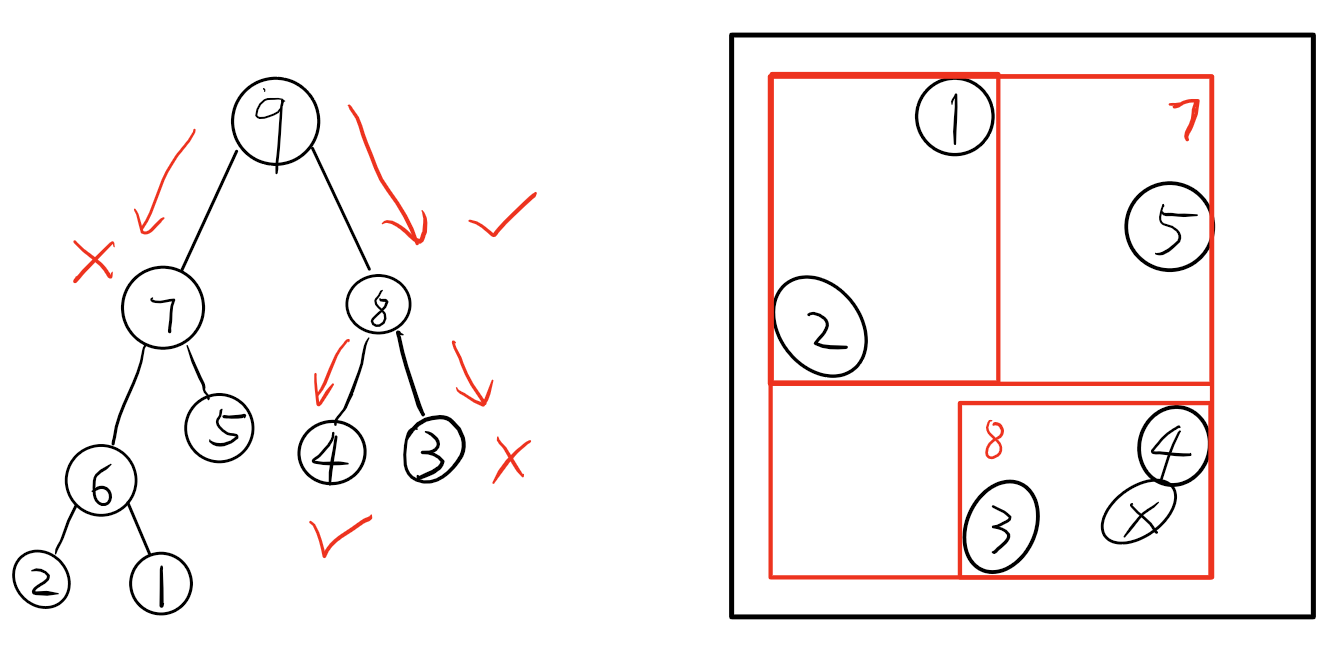
\includegraphics[width=10cm]{./rep_8.png}
\caption{Top-down BVH tree traversal for one object x. When it goes to the AABB of node 7, there is not an intersection. Therefore it skips node 7. Then it finds out it has an intersection with the AABB of node 8, so it traverses down the node 8. Finally, it goes to node 4. We can parallelize this procedure by making processors have each object traverse the tree simultaneously.}
\end{figure}

Since the nearby objects tend to be grouped together in the same subtree by z-ordering, the parallel traversal is also cache-friendly because nearby threads are usually accessing nearby memory.

\subsubsection{Narrow Phase Collision Detection}
\label{sec:org15c421f}

Theoretically, a narrow phase detection procedure is used to determine two objects are colliding. Since I only consider sphere objects in the project to simplify the problem, the shape information of objects are omitted, and I use the distance between sphere pairs and their radius sums to determine whether they are intersecting or not. This part can be further improved in my future game engine development work.

Also, in this phase, I directly resolve the collision by modifying the dynamics attribute for each colliding object pair. I combine the narrow phase detection the collision resolution to simplify the program implementation. In general industrial applications, it is better to focus on broad phase detection because it can substantially reduce the work in next steps.

\subsubsection{Solution Summary}
\label{sec:org93030bc}
To sum up, we now have a simulation pipeline like the following:
\begin{figure}[htbp]
\centering
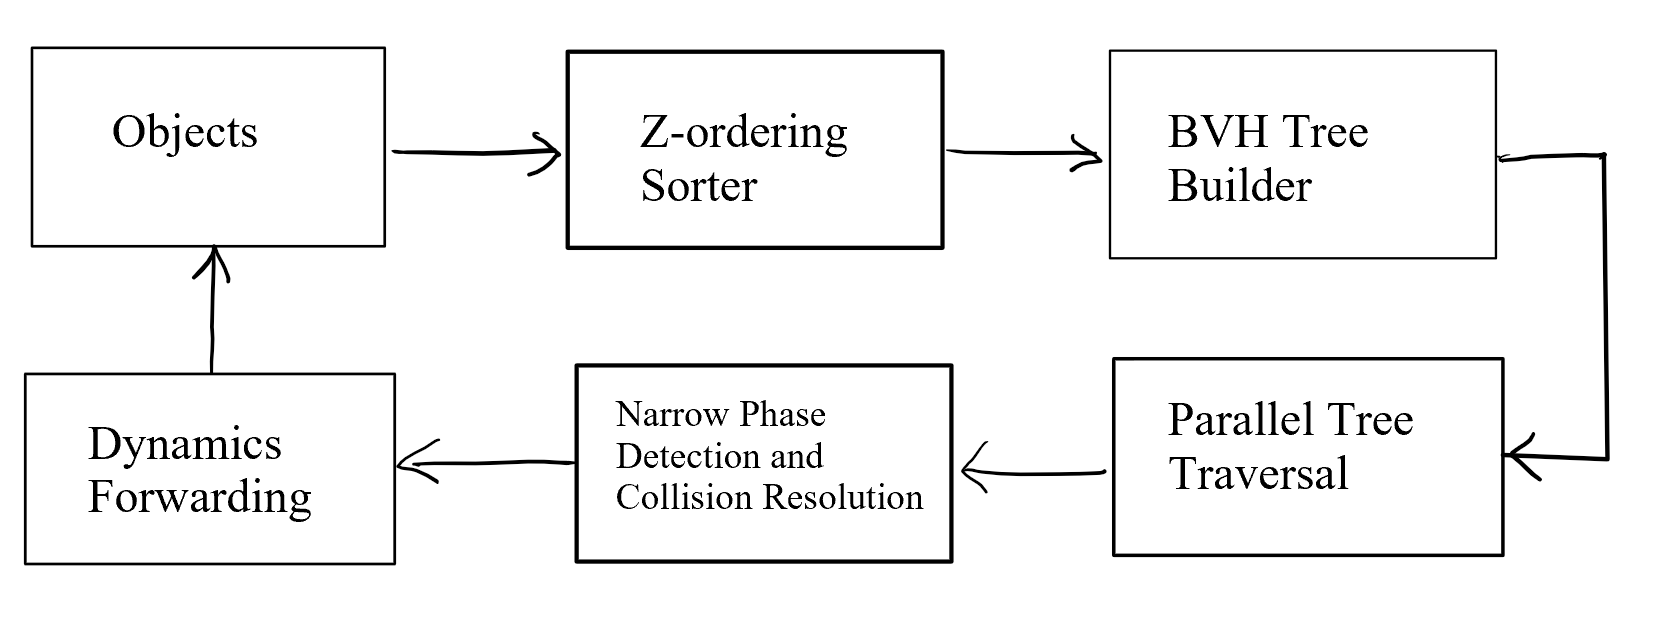
\includegraphics[width=.9\linewidth]{./rep_9.png}
\caption{Simulation pipeline (or circle).}
\end{figure}

\section{Performance Measurement}
\label{sec:org9af44c1}
Firstly I would list the performance of dynamics forwarding phase:

\begin{table}[htbp]
\centering
\begin{tabular}{rrrrrrrrr}
Objects(N) & Blocks(B) & Threads(T)/B & Time(ms) & Speedup & B & T/B & Time(ms) & S\\
\hline
1000 & 2 & 4 & 0.122720 & 1 & 4 & 4 & 0.071584 & 1.71\\
 & 4 & 8 & 0.032768 & 3.74 & 8 & 8 & 0.019296 & 6.36\\
 & 8 & 16 & 0.013248 & 9.26 & 16 & 16 & 0.009472 & 12.96\\
\hline
5000 & 2 & 4 & 0.535296 & 1 & 4 & 4 & 0.266784 & 2.01\\
 & 4 & 8 & 0.145792 & 3.67 & 8 & 8 & 0.085216 & 6.28\\
 & 8 & 16 & 0.052512 & 10.19 & 16 & 16 & 0.024456 & 21.89\\
\hline
10000 & 2 & 4 & 1.05216 & 1 & 4 & 4 & 0.536256 & 1.96\\
 & 4 & 8 & 0.268928 & 3.91 & 8 & 8 & 0.149824 & 7.02\\
 & 8 & 16 & 0.088224 & 11.93 & 16 & 16 & 0.042528 & 24.74\\
\hline
50000 & 2 & 4 & 6.19203 & 1 & 4 & 4 & 3.09773 & 2.00\\
 & 4 & 8 & 1.57142 & 3.94 & 8 & 8 & 0.795168 & 7.79\\
 & 8 & 16 & 0.408704 & 15.15 & 16 & 16 & 0.218240 & 28.37\\
\end{tabular}
\caption{Dynamics forwarding performance. Measured on Nvidia\textregistered GTX 940M (384 shading units, each 1072MHz). Parallelization achieved using CUDA 8.0 framework.}

\end{table}

Then I will provide a brief table showing the performance of Lauterbach and Luebke(2007) method in "Box Collider" environment.


\begin{table}[H]
\centering
\begin{tabular}{rrrrrrrrr}
Objects(N) & Blocks(B) & Threads(T)/B & Time(ms) & Speedup & B & T/B & Time(ms) & S\\
\hline
10000 & 2 & 4 & 22.83467 & 1 & 4 & 4 & 13.57422 & 1.68\\
 & 4 & 8 & 9.623959 & 2.37 & 8 & 8 & 6.859251 & 3.33\\
 & 8 & 16 & 4.478128 & 5.10 & 16 & 16 & 3.148109 & 7.25\\
\end{tabular}
\caption{Collision handling performance (using the original paper's method). Measured on Nvidia\textregistered GTX 940M (384 shading units, each 1072MHz). Parallelization achieved using CUDA 8.0 framework.}

\end{table}

The following is the performance of collision handling process when we use bottom-up approach to construct BVH.

\begin{table}[H]
\centering
\begin{tabular}{rrrrrrrrr}
Objects(N) & Blocks(B) & Threads(T)/B & Time(ms) & Speedup & B & T/B & Time(ms) & S\\
\hline
1000 & 2 & 4 & 1.02256 & 1 & 4 & 4 & 0.600480 & 1.70\\
 & 4 & 8 & 0.383522 & 2.67 & 8 & 8 & 0.195681 & 5.23\\
 & 8 & 16 & 0.136486 & 7.49 & 16 & 16 & 0.103849 & 9.85\\
\hline
5000 & 2 & 4 & 4.88496 & 1 & 4 & 4 & 2.50912 & 1.95\\
 & 4 & 8 & 1.40656 & 3.47 & 8 & 8 & 0.738243 & 6.62\\
 & 8 & 16 & 0.456867 & 10.69 & 16 & 16 & 0.240884 & 20.28\\
\hline
10000 & 2 & 4 & 9.46384 & 1 & 4 & 4 & 4.87392 & 1.94\\
 & 4 & 8 & 2.59872 & 3.64 & 8 & 8 & 1.41523 & 6.69\\
 & 8 & 16 & 0.775528 & 12.20 & 16 & 16 & 0.457289 & 20.70\\
\hline
50000 & 2 & 4 & 56.4363 & 1 & 4 & 4 & 28.3112 & 1.99\\
 & 4 & 8 & 14.5653 & 3.87 & 8 & 8 & 7.55952 & 7.47\\
 & 8 & 16 & 4.01712 & 14.05 & 16 & 16 & 2.16896 & 26.02\\
\end{tabular}
\caption{Collision handling performance (using the bottom-up tree construction). Measured on Nvidia\textregistered GTX 940M (384 shading units, each 1072MHz). Parallelization achieved using CUDA 8.0 framework.}

\end{table}

Finally, the first and the third table is added up to show the total time for each frame.

\begin{table}[H]
\centering
\begin{tabular}{rrrrrrrrr}
Objects(N) & Blocks(B) & Threads(T)/B & Time(ms) & Speedup & B & T/B & Time(ms) & S\\
\hline
1000 & 2 & 4 & 1.14528 & 1 & 4 & 4 & 0.672064 & 1.70\\
 & 4 & 8 & 0.41629 & 2.75 & 8 & 8 & 0.214977 & 5.33\\
 & 8 & 16 & 0.149734 & 7.65 & 16 & 16 & 0.113321 & 10.11\\
\hline
5000 & 2 & 4 & 5.420256 & 1 & 4 & 4 & 2.775904 & 1.95\\
 & 4 & 8 & 1.552352 & 3.49 & 8 & 8 & 0.823459 & 6.58\\
 & 8 & 16 & 0.509379 & 10.64 & 16 & 16 & 0.26534 & 20.43\\
\hline
10000 & 2 & 4 & 10.516 & 1 & 4 & 4 & 5.410176 & 1.94\\
 & 4 & 8 & 2.867648 & 3.67 & 8 & 8 & 1.565054 & 6.72\\
 & 8 & 16 & 0.863752 & 12.17 & 16 & 16 & 0.499817 & 21.04\\
\hline
50000 & 2 & 4 & 62.62833 & 1 & 4 & 4 & 31.40893 & 1.99\\
 & 4 & 8 & 16.13672 & 3.88 & 8 & 8 & 8.354688 & 7.50\\
 & 8 & 16 & 4.425824 & 14.15 & 16 & 16 & 2.3872 & 26.24\\
\end{tabular}
\caption{Dynamics forwarding + collision handling performance (using the bottom-up tree construction). Measured on Nvidia\textregistered GTX 940M (384 shading units, each 1072MHz). Parallelization achieved using CUDA 8.0 framework.}

\end{table}

\subsection{Analysis}
\label{sec:orga07f00b}
We can analyze the result in two aspects. Firstly, I would call the scaling of the simulation pipeline "moderate," since it has the efficiency of 80\% in most cases. While GPU programming usually suffers from poor efficiency, this performance seems good enough. However, considering the problem I am solving, I think there is better way to make the speedup linear. The medium speedup should be ascribed to the GPU radix sorting method I used in this project, as it requires to frequently transfer data between threads in different blocks of the GPU, which is a common challenge especially when the memory of each block and thread are limited. The sorting algorithm seems to be the main factor that eats up the speedup. In regular computer games, this cost is affordable because there are no more than 10000 objects in one scene and the frequency is usually 60Hz, which means we need to update the state of objects every 16ms. In our benchmark, with 128 shading units, we can already limit the cost of simulation from 0ms to 4ms. Therefore this work is somehow applicable to a real-world game engine.

Secondly, we can notice an interesting point that as the size of input N goes up, the simulation program will be more likely to converge to the status of linear speedup. I think the reason is that the work is more balanced in the "bottom-up" tree construction phase when the number of objects is large, because when there are more objects, the relatively less time for idling threads to spend on waiting when we are close to the tree root. Therefore I expect this pipeline to perform even better on larger input size.

\section{Summary}
\label{sec:org631426c}
In this report, I present my procedure of conceiving and implementing a GPU-accelerated rigid body simulator. In the beginning, I determined the representation for dynamics and shape attribute of a rigid body respectively, then put my concentration on balancing the work of collision handling among GPU processing units. When tried to implement a tree construction procedure, I found a well-established approach is not entirely suitable for my benchmark. Therefore another way of constructing BVH trees is used here as a substitution to the original implementation. I would treat this method as a bottom-up way for building trees. Finally, I did performance measurement on this pipeline and found fascinating results.
I would like to say that this project changes my way of thinking. I knew GPU-accelerated programs sometimes could be super fast, but only when I started to programming for a GPU myself I know the interesting part is not only the performance, it is more about thinking in parallel. In this project, I use a lot of program implementation that would be considered pretty slow in serial condition, but they turned out to be faster when it comes to GPU environment. I think I would be very interested in improving the performance and stability of this physics engine further in the future.

\section{Furture Work}
\label{sec:orge4ece62}
\subsection{More Algorithm Implementation}
\label{sec:orgb6e99a1}
In this project, I simplified a lot of work on narrow phase collision detection. There is a quite famous algorithm called "GJK" algorithm that detects collision by calculating the Minkowski difference between two shapes, which is also interesting to parallelize in my future work. Also, mature physics engines always offer constraint enforcement mechanism to help developers to construct complex physics scenes, like spring system and so on. Because I have many other things to do this semester, these features should be considered in the future, maybe next year.
\subsection{Integration with My Game Engine}
\label{sec:orgb51250d}
Currently, this simulation system has no well-designed software interface; therefore I also would like to think more about how to expose a set of reasonable application interface so that it integrates well with the game engine I am currently developing.

\section{Core References}
\label{sec:org8004b10}
Baraff, David. "An introduction to physically based modeling: rigid body simulation I—unconstrained rigid body dynamics." SIGGRAPH Course Notes (1997).
\\
\\
Lauterbach, Christian, et al. "Fast BVH construction on GPUs." Computer Graphics Forum. Vol. 28. No. 2. Blackwell Publishing Ltd, 2009.
\\
\\
"Thinking Parallel, Part II: Tree Traversal on the GPU" Tero Karras, 26 Nov. 2012, \url{https://devblogs.nvidia.com/parallelforall/thinking-parallel-part-ii-tree-traversal-gpu/}
\end{document}